\chapter{Điều khiển phần cứng qua các chân GPIO}
\section{Giới thiệu}
Ngoài chức năng như một máy tính mini (dùng để học tập, giải trí,\ldots), Raspberry Pi còn có khả năng giao tiếp và điều khiển các phần cứng khác (cảm biến, các module mở rộng khác, động cơ, giao tiếp với các IC khác,\ldots) thông qua các chân GPIO.\\

Số chân GPIO tùy thuộc vào từng phiên bản Raspberry Pi: có hai loại là 26 chân GPIO (model A, B) và 40 chân GPIO (model A+, B+, Pi 2, Pi 3, PiZero).
\begin{figure}[!h]
%\begin{center}
	\subfloat[Model 26 pin GPIO]
	{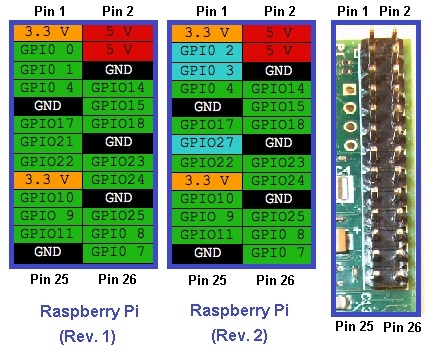
\includegraphics[scale=.6]{GPIO/images/PiA}}\hspace{2cm}
	\subfloat[Model 40 pin GPIO]
	{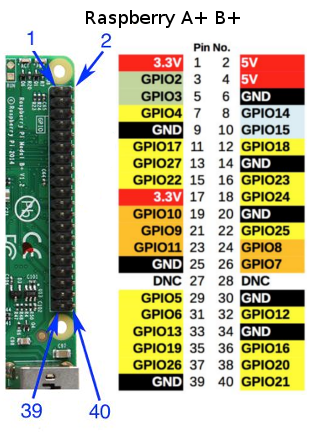
\includegraphics[scale=.6]{GPIO/images/PiB}}
%\end{center}
\caption{Số chân GPIO của các phiên bản Raspberry Pi}\label{Fig:gpio}
\end{figure}
\section{Mô tả chức năng của các nhóm chân}
Trên Raspberry Pi sẽ có các nhóm chân sau đây (ta sẽ sử dụng cách đánh số từ $1 \rightarrow 40$ như trên hình \ref{Fig:gpio}):
\begin{itemize}
\item \textit{Nhóm chân cấp nguồn:}
\begin{itemize}
\item Nguồn 5V: gồm 2 chân -- số 2 và 4.
\item Nguồn 3.3V: gồm 2 chân -- số 1 và 17.
\item Chân GND: gồm 5 chân -- số $6,9,14,25$ (Model 26 chân) hoặc gồm 8 chân -- số $6,9,14,25,30,$ $34,39$ (Model 40 chân).
\end{itemize}
\item \textit{Nhóm chân GPIO (I/O):}
\begin{itemize}
\item Model 26 chân: gồm 8 chân -- số $7, 11, 12, 13, 15, 16, 18, 22$.
\item Model 40 chân: gồm 17 chân -- số $7, 11, 12, 13, 15, 16, 18, 22, 29, 31, 32, 33, 35, 36,$ $37, 38, 40$.
\end{itemize}
\item \textit{Chân PWM -- Pulse Width Modulation}: gồm 2 chân -- chân số 12 và 13.
\item \textit{Nhóm chân giao tiếp $I2C$}: gồm 2 chân -- số 3 và 5.\\
Ta có thể điều khiển nhiều thiết bị I2C chỉ với 2 chân này, mỗi thiết bị sẽ được phân biệt bởi một địa chỉ riêng của nó. Cần khai báo đúng địa chỉ của thiết bị cần điều khiển.
\item \textit{Nhóm chân giao tiếp $SPI$:} gồm 5 chân -- số $19, 21, 23, 24, 26$.
\item \textit{Nhóm chân giao tiếp UART}: gồm 2 chân -- số 8 và số 10.
\item \textit{Nhóm chân giao tiếp EEPROM:} gồm 2 chân -- số 27 và 28 (chỉ có ở model Pi có 40 chân GPIO).
\end{itemize}
\section{Các cài đặt và cấu hình cần thiết để sử dụng được các chân GPIO}
Trong bài viết mình sẽ chọn ngôn ngữ lập trình Python (Phython 2) để điều khiển các chân GPIO của Raspberry Pi. Những dọng lệnh bên dưới, sẽ được thực hiện trên của sổ dòng lệnh.
\subsection{Cài đặt thư viện RPi.GPIO}
Gõ lệnh sau: \verb|sudo apt-get install python-dev python-rpi.gpio|
\subsection{Xác nhận cấu hình I2C}\label{Sub:I2C}
Chỉ khi nào giao tiếp I2C thì mới thực hiện \textit{mục \ref{Sub:I2C}}.

Gõ lệnh sau: \verb|sudo apt-get install python-smbus i2c-tools|

Chạy \verb|sudo raspi-config| để Enable I2C (thường khi cài đặt hệ điều hành thì I2C ở chế độ Disable).

Thực hiện theo các bước từ \textit{hình \ref{Fig:start}} đến \textit{hình \ref{Fig:reset}} trong \textit{hình \ref{Fig:I2C}}. Sau khi thực hiện bước cuối cùng trong \textit{hình \ref{Fig:reset}}, Raspberry Pi sẽ reset lại.
\begin{figure}
	\subfloat[Chọn \textsf{8 Advance Options} rồi \textsf{Enter}\label{Fig:start} ]
	{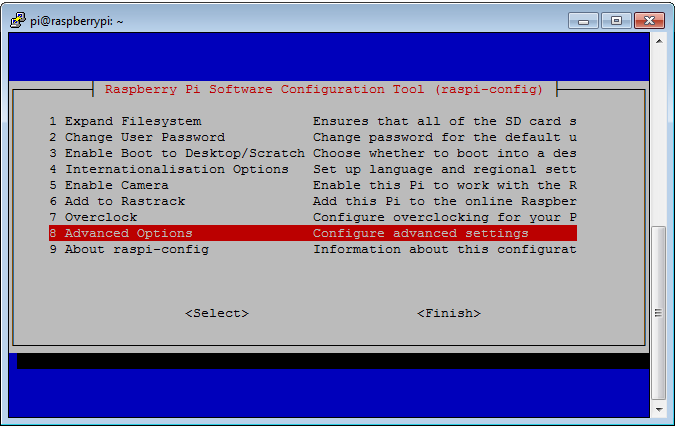
\includegraphics[scale=.45]{GPIO/images/raspi-1}}\hspace{1cm}
	\subfloat[Chọn \textsf{A7 I2C} rồi \textsf{Enter}\label{Fig:b2}]
	{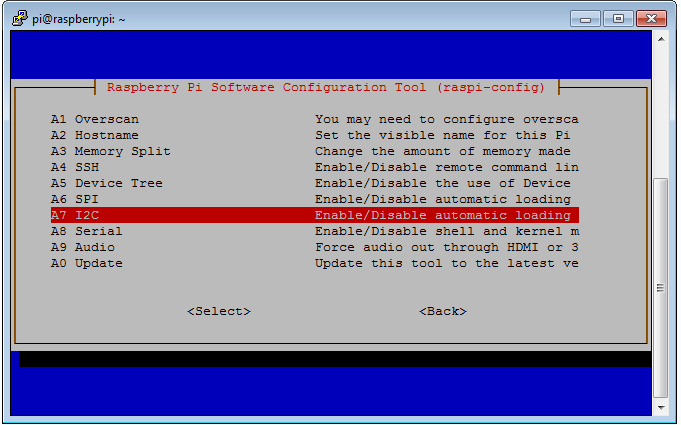
\includegraphics[scale=.45]{GPIO/images/raspi-2}}\\
	\subfloat[Chọn \textsf{Yes} rồi \textsf{Enter}]
	{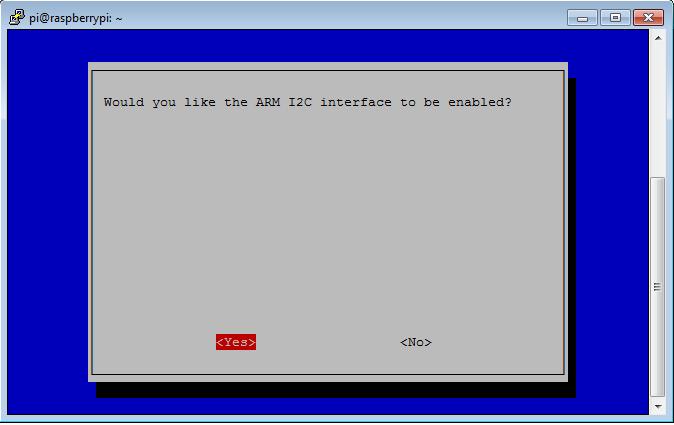
\includegraphics[scale=.45]{GPIO/images/raspi-3}}\hspace{1cm}
	\subfloat[Chọn \textsf{OK} rồi \textsf{Enter}]
	{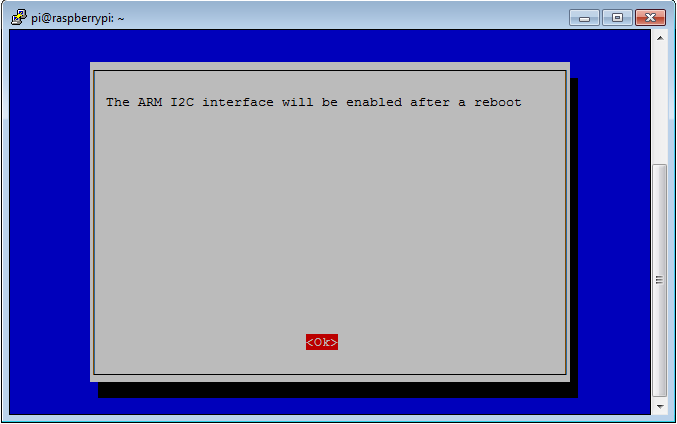
\includegraphics[scale=.45]{GPIO/images/raspi-4}}\\
	\subfloat[Chọn \textsf{Yes} rồi \textsf{Enter}]
	{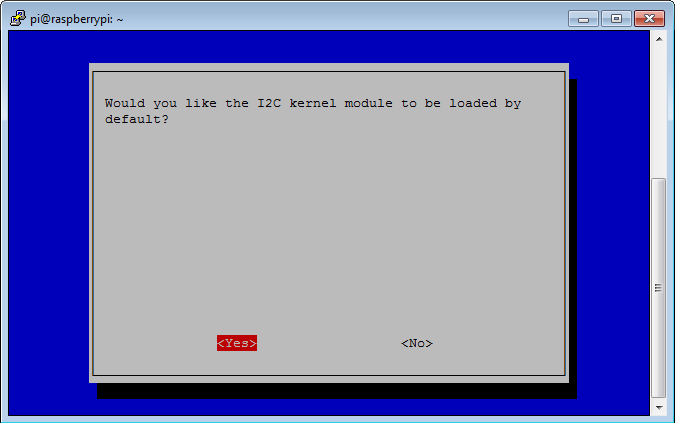
\includegraphics[scale=.45]{GPIO/images/raspi-5}}\hspace{1cm}
	\subfloat[Chọn \textsf{OK} rồi \textsf{Enter}]
	{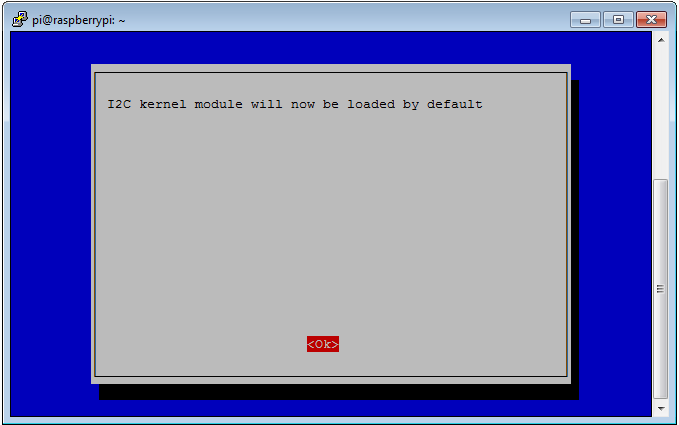
\includegraphics[scale=.45]{GPIO/images/raspi-6}}\\
	\subfloat[Chọn \textsf{Finish} rồi \textsf{Enter}]
	{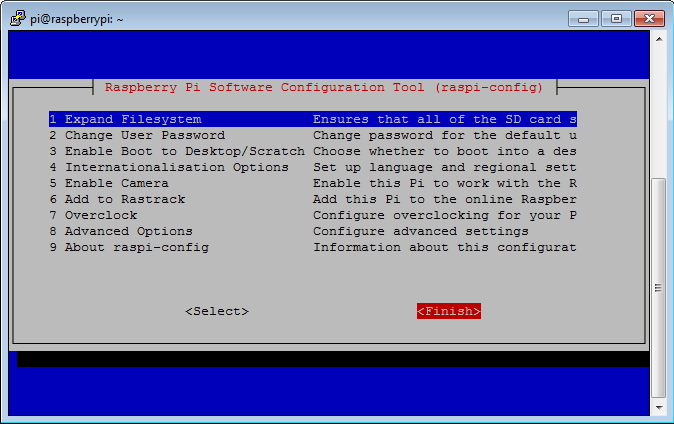
\includegraphics[scale=.45]{GPIO/images/raspi-7}}\hspace{1cm}
	\subfloat[Chọn \textsf{Yes} rồi \textsf{Enter}\label{Fig:reset}]
	{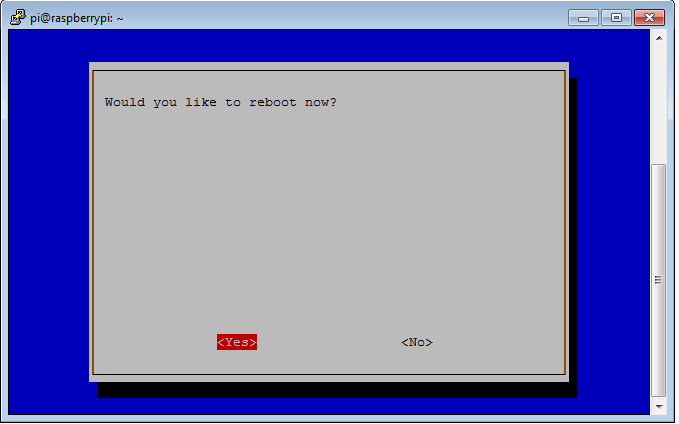
\includegraphics[scale=.45]{GPIO/images/raspi-8}}\\
	
\caption{Cách cấu hình I2C trên Raspberry Pi} \label{Fig:I2C}
\end{figure}
Khi Raspberry Pi khởi động trở lại, ta thực hiện, tiếp:
\begin{itemize}
\item Mở file \verb|modules|, dùng lệnh: \verb|sudo nano /etc/modules|
\item Thêm vào file \verb|moludes| với nội dụng giống như hình bên dưới: thêm vào 2 dòng \verb|i2c-bcm2708| và \verb|i2c-dev| (Nhấn Ctrl + X + Y để lưu file và thoát khỏi).
\begin{figure}[!h]
\begin{center}
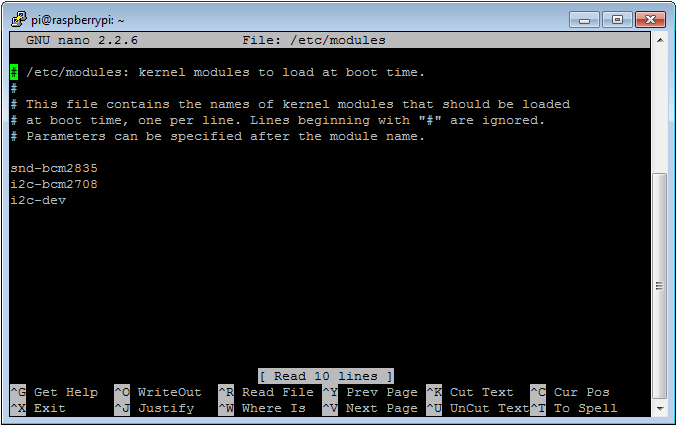
\includegraphics[scale=.5]{GPIO/images/raspi-9}
\end{center}
\end{figure}
\item Mở file \verb|raspi-blacklist.conf|, dùng lệnh:
\begin{center}
\verb|sudo nano /etc/modprobe.d/raspi-blacklist.conf|
\end{center}
\item Thêm dấu \verb|#| vào trước 2 dòng: \verb|blacklist spi-bcm2708| và \verb|blacklist i2c-bcm2708| (Nhấn Ctrl + X + Y để lưu file và thoát khỏi).
\begin{figure}[!h]
\begin{center}
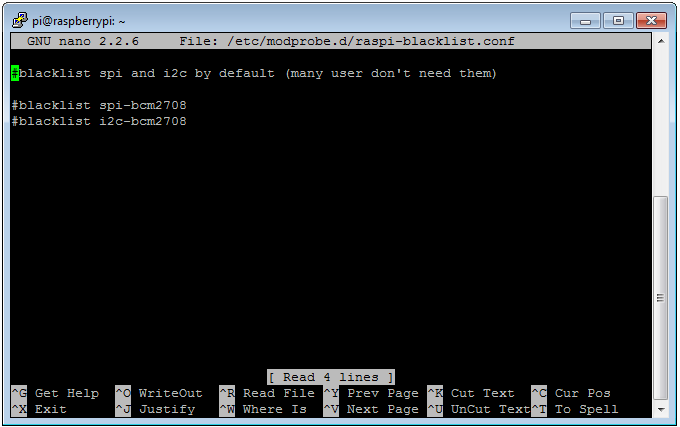
\includegraphics[scale=.5]{GPIO/images/raspi-10}
\end{center}
\end{figure}
\item Sau khi thực xong, chúng ta reset lại Raspberry Pi: \verb|sudo reboot|
\end{itemize} 
\subsection{Xác nhận cấu hình SPI}\label{Sub:SPI}
Chỉ khi nào giao tiếp SPI thì mới thực hiện \textit{mục \ref{Sub:SPI}}.\\

Thực hiện \verb|Enable| SPI với lệnh \verb|sudo raspi-config|, tương tự như \verb|Enable| I2C (đến \textit{hình \ref{Fig:b2}} ta chọn \verb|A6 SPI|).\\

Khi Raspberry Pi khởi động trở lại, ta thực hiện:
\begin{itemize}
\item Mở file \verb|raspi-blacklist.conf|, dùng lệnh:
\begin{center}
\verb|sudo nano /etc/modprobe.d/raspi-blacklist.conf|
\end{center}
\item Thêm dấu \verb|#| vào trước 2 dòng: \verb|blacklist spi-bcm2708| và \verb|blacklist i2c-bcm2708| (Nhấn Ctrl + X + Y để lưu file và thoát khỏi). Nếu không có file này thì hãy tạo lại với nội dung như bên dưới.
\end{itemize}
\section{Sử dụng các chân GPIO để điều khiển phần cứng cùng với ngôn ngữ lập trình Python}
Phần này dựa vào bài viết của tác giả: \textsf{Anonymous} với chủ đề:

\textit{raspberry-gpio-python -- A Python module to control the GPIO on a Raspberry Pi} \footnote{\textsf{https://sourceforge.net/p/raspberry-gpio-python/wiki/Examples/}}\\

Hiện tại thì thư viện này chưa hổ trợ các giao tiếp SPI, I2C, 1-wire, chúng ta chỉ sử dụng nó với các lệnh cơ bản bên dưới.

Tránh đặt điện áp lớn hơn 3.3V vào trực tiếp các chân GPIO vì sẽ làm hỏng chúng.
\subsection{Kiểm tra chức năng của các chân GPIO}
Sử dụng các chân GPIO trên Raspberry Pi phải đúng với chức năng của nó thì mới đem lại hiệu quả.
\begin{itemize}
\item Kiểm tra chức năng của từng chân:
\begin{lstlisting}[language=Python]
import RPi.GPIO as GPIO

GPIO.setmode(GPIO.BOARD)
func = GPIO.gpio_function(pin)
\end{lstlisting}
\item Kết quả trả về là: \verb|GPIO.IN|, \verb|GPIO.OUT|, \verb|GPIO.SPI|, \verb|GPIO.I2C|, \verb|GPIO.HARD_PWM|, \verb|GPIO.SERIAL|, \verb|GPIO.UNKNOWN|
\end{itemize}
\subsection{Các lệnh cơ bản trong thư viện RPi.GPIO}
%\lstinputlisting[language=Python]{import.py}
\begin{itemize}
\item Khai báo thư viện \verb|RPi.GPIO|:
\begin{lstlisting}[language=Python]
import RPi.GPIO as GPIO #Dung ten GPIO thay cho RPi.GPIO
\end{lstlisting}
Kiểm tra thông tin về Pi và chân GPIO:
\begin{lstlisting}[language=Python]
GPIO.RPI_INFO
#Ket qua tra ve: P1_REVISION; RAM; REVISION; TYPE; PROCESSOR; MANUFACTURER
#Vi du: {'P1_REVISION': 3, 'RAM': '512M', 'REVISION': '0010', 'TYPE': 'Model B+', 'PROCESSOR': 'BCM2835', 'MANUFACTURER': 'Unknown'}
#Ta co the dung lenh: GPIO.RPI_INFO[Tham so] de xem mot thong so quan tam

#Dung lenh: GPIO.RPI_REVISION de xem phien ban chan GPIO 
GPIO.VERSION #Kiem tra phien ban GPIO
#Vi du: '0.6.2'
\end{lstlisting}
\item Xác định cách khai báo số chân là \verb|GPIO.BOARD| hay \verb|GPIO.BCM|:
\begin{lstlisting}[language=Python]
GPIO.setmode(GPIO.BOARD) #Danh so chan theo so tren Board tu so 1 den so 40
GPIO.setmode(GPIO.BCM) #Danh so chan theo ten GPIO, vi du GPIO27, GIPO14,...
\end{lstlisting}
Để kiểm tra xem bạn đang sử dụng cách khai báo nào trong 2 cách khai báo \verb|BOARD| hoặc \verb|BCM|, dùng lệnh sau:
\begin{lstlisting}[language=Python]
mode = GPIO.getmode() #Xem khai bao BOARD hoac BCM
print mode  
#mode = -1: chua khai bao
#mode = 10: khai bao la BOARD
#mode = 11: khai bao la BCM
\end{lstlisting}
\item Khi các chân GPIO đã được sử dụng trước đó (chưa được cleanup) thì sử dụng lại chương trình sẽ thông báo các cảnh báo, ta sử dụng lệnh sau để vô hiệu cảnh báo:
\begin{lstlisting}[language=Python]
GPIO.setwarnings(False) #Bo qua cac canh bao ve GIPO
\end{lstlisting}
\item Khai báo chân GPIO cần điều khiển là chân \verb|input| hay chân \verb|output|:
\begin{lstlisting}[language=Python]
#pin la chan GPIO can dieu khien
GPIO.setup(pin, GPIO.IN) #Khai bao pin chan INPUT
GPIO.setup(pin, GPIO.OUT) #Khai bao pin chan OUTPUT


#Khi can khai bao nhieu chan INPUT va OUTPUT
pin_input = [pin1, pin2, pin2] #Danh sach cac chan INPUT
pin_output = [pin4, pin4, pin6] #Danh sach cac chan OUTPUT

GPIO.setup(pin_input, GPIO.OUT) #Khai bao nhieu chan la INPUT
GPIO.setup(pin_output, GPIO.OUT) #Khai bao nhieu chan la OUTPUT
\end{lstlisting}
\item Với một số ứng dụng ta cần \textit{mắc điện trở treo (lên nguồn hoặc nối mass)}: có thể làm việc này bằng phần cứng hoặc bằng phần mềm. Ở đây ta sử dụng phần mềm.
\begin{lstlisting}[language=Python]
#pin1, pin2 la chan GPIO can dieu khien

#Khai bao pin chan INPUT, co dien tro mac len nguon - 3.3V
GPIO.setup(pin1, GPIO.IN,pull_up_down = GPIO.PUD_UP) 

#Khai bao pin chan INPUP, co dien tro mac xuong mass - 0V
GPIO.setup(pin2, GPIO.IN, pull_up_down = GPIO.PUD_DOWN) 
\end{lstlisting}
\item Đọc tín hiệu từ chân \verb|INPUT|:
\begin{lstlisting}[language=Python]
#pin la chan GPIO can dieu khien
read_input = GPIO.input(pin) #Doc tin hieu cua chan INPUT
#read_input la 0 hoac 1 hoac GIPO.LOW hoac GPIO.HIGH hoac False hoac True
\end{lstlisting}
\item Xuất tín hiệu ra chân GPIO là chân \verb|OUTPUT|:
\begin{lstlisting}[language=Python]
#pin la chan OUTPUT

#Co 3 cach xuat chan GPIO pin ra muc cao
GPIO.output(pin,1)
GPIO.output(pin,True) 
GPIO.output(pin,GPIO.HIGH) 

#Co 3 cach xuat chan GPIO pin ra muc thap
GPIO.output(pin,0)
GPIO.output(pin,False) 
GPIO.output(pin,GPIO.LOW)

#Khi can xuat tin hieu ra nhieu chan
pin_output = [pin1, pin2, pin3] #Danh sach cac chan OUTPUT
GPIO.output(pin_output,0) #Cac pin o muc thap, 
GPIO.output(pin_output,0) #Cac pin o cao
#Co the su dung tham so: 0, 1 hoac False, True hoac GPIO.LOW, GPIO.HIGH 

#Ham Output va Input ket hop voi nhau
#Doc gia tin hieu tu 1 chan va xuat no ra chinh no pin
GPIO.output(pin, not GPIO.input(pin))
\end{lstlisting}
\item Kết thúc quá trình làm việc với các chân GPIO, có 2 tùy chọn:
\begin{lstlisting}[language=Python]
GPIO.cleanup() #clear tat ca cac chan GPIO
GPIO.cleanup([pin_1, pin_2]) #Chi clear mot so chan GPIO
\end{lstlisting}
\end{itemize}
\subsection{Ngắt và phát hiện tín hiệu cạnh}
\textit{Ngắt} là bắt chương trình dừng công việc đang thực hiện để thực hiện một công việc khác.

\textit{Tín hiệu cạnh} là tín hiệu số biến đổi từ mức thấp lên mức cao ($0 \rightarrow 1$) hoặc từ mức cao xuống mức thấp ($1 \rightarrow 0$).
\begin{itemize}
\item Hàm \verb|wait_for_edge()|: thực hiện chương trình khi phát hiện được tín hiệu cạnh.
\begin{lstlisting}[language=Python]
#Phat hien tin hieu canh o chan GPIO pin
GPIO.wait_for_edge(pin, GPIO.RISING)  #RISING chuyen tu 0 len 1
GPIO.wait_for_edge(pin, GPIO.FALLING)  #FALLING chuyen tu 1 xuong 0
GPIO.wait_for_edge(pin, GPIO.BOTH)  #BOTH chi can co tin hieu canh
#GPIO.BOTH gom GPIO.RISING va GPIO.FALLING

#Khi can doi tin hieu canh trong thoi gian nhat dinh
#Doi tin hieu canh (RISING,FALLING, BOTH) trong thoi gian timeout = t
#Don vi cua t la ms, vi du: timeout = 5000 (t = 5s)
#Neu qua thoi gian timeout ma khong phat hien canh thi ket qua la None

#Doi canh chuyen tu 0 len 1 voi thoi gian t (ms)
signal_edge  = GPIO.wait_for_edge(pin, GPIO.RISING, timeout=t) 

#Doi canh chuyen tu 1 len 0 voi thoi gian t (ms)
signal_edge  = GPIO.wait_for_edge(pin, GPIO.FALLING, timeout=t) 

#Doi tin hieu canh voi thoi gian t (ms)
signal_edge  = GPIO.wait_for_edge(pin, GPIO.BOTH, timeout=t) 
\end{lstlisting}
\item Hàm \verb|event_detected()|: khi chương trình đang thực hiện một công việc nào đó, nếu có tín hiệu cạnh thì nó sẽ nhảy sang một việc khác.
\begin{lstlisting}[language=Python]
GPIO.add_event_detect(pin, GPIO.RISING) #FALLING, BOTH
#Phat hien tin hieu canh tu 0 len 1
#
#Cong viec dan thuc hien vi du: trong vong lap for, while,...
#
if GPIO.event_detected(channel):
	print "Thuc hien chuong trinh o phan nay"
\end{lstlisting}
\item Dùng chức năng phát hiện cạnh thì nhảy sang \textit{chương trình ngắt} được định nghĩa trước để thực hiện câu lệnh.
\begin{lstlisting}[language=Python]
def chuong_trinh_ngat_1():
	#
	#Noi dung can thuc hien khi co ngat
	#

def chuong_trinh_ngat_2():
	#
	#Noi dung can thuc hien khi co ngat
	#
GPIO.add_event_detect(pin, GPIO.RISING) #FALLING, BOTH
GPIO.add_event_callback(pin, chuong_trinh_ngat_1())
GPIO.add_event_callback(pin, chuong_trinh_ngat_2())

#Them vao tham so bouncetime = t(ms) de chong nhieu
GPIO.add_event_callback(pin, chuong_trinh_ngat_1, bouncetime=t)
GPIO.add_event_callback(pin, chuong_trinh_ngat_2, bouncetime=t)
\end{lstlisting}
\item Hàm \verb|remove_event_detect()|: không sử dụng chức của hàm \verb|event_detected()| nữa.
\begin{lstlisting}[language=Python]
GPIO.remove_event_detect(pin) #pin GPIO duoc su dung voi ngat truoc do
\end{lstlisting}
\end{itemize}
\subsection{Sử dụng chân GPIO với chức năng PWM}
Ta thực hiện theo các bước:
\begin{itemize}
\item Khởi tạo một khối PWM:
\begin{lstlisting}[language=Python]
p = GPIO.PWM(channel, freq)
#channel: chan so 12 va so 13 hoac GPIO18 va GPIO27
#freq: tan so xung vuong
\end{lstlisting}
\item Bắt đầu với PWM:
\begin{lstlisting}[language=Python]
p.start(duty_cycle)
#duty_cycle = T_on/T = T_on/(T_on T_off) = 0 - 100%
\end{lstlisting}
\item Lệnh thay đổi tần số và chu kỳ:
\begin{lstlisting}[language=Python]
#Thay doi tan so
p.ChangeFrequency(freq) #freq: la tan so moi

#Thay doi phan tram T_on
p.ChangeDutyCycle(duty_cycle) #duty_cycle: phan tram T_on moi
\end{lstlisting}
\item Dừng khối PWM:
\begin{lstlisting}[language=Python]
p.stop() #Dung khoi PWM voi ten bien la p
\end{lstlisting}
\end{itemize}
%\subsection{Các lệnh trong thư viện RPi.GPIO}